\chapter{Methods}\label{ch:methods}

The last chapter introduced Gaussian process regression to establish a mapping
between a time point $x$ and its corresponding BP value. Since Gaussian Processes
are capable of modeling time series in continuous time and hence deal with
irregularly spaced data, they seem to be a good candidate for modeling a time
series from which we only have irregularly sampled noisy measurements.

This chapter outlines the methodology for evaluating the performance of Gaussian
process regression and baseline methods for estimating blood pressure values from
noisy measurements. It also discusses the analysis of adversarial factors that may
affect estimation accuracy.


%Additionally, the impact of different adversarial factors on the target measure
%estimate should be investigated. This will be described in section
%\ref{sec:adversarial-analysis}.



\section{Problem Statement}

Recall the problem statement from section \ref{sec:problem-statement}. First, we
assumed the following model for the BP measurements $Y(x)$ at a time point $x$:

\begin{align*}
    Y(x) = f(x) + \epsilon && \epsilon \sim \N(0, \sigma_n^{2})
\end{align*}

where $f(x)$ denotes the true BP process and $\epsilon$ is iid measurement noise,
independent from $f(x)$.

The goal is to estimate the true BP values $f(x)$ at some input time $X$,
based on noisy observations of $f(x)$ at some training time points $X_{train}$.
For the sections of this chapter, we define:

\begin{itemize}
    \item $X := \{ x_1, \dots, x_n \}$: An index set spanning the one-week time
    range of interest, with 10 BP values per hour.
    It defines the time points at
    which we want to predict BP values and hence represents the regression input.

    \item $X_{train} \subset X$: The training indexes. \\

    \item $G_X := (g(x) : x \in X )$ for some function $g(x)$.
    Specifically:
    \begin{description}
        \item $F_X := (f(x) : x \in X)$: The true BP values at inputs $X$.
        \item $Y_X = (Y(x) : x \in X)$: The noisy BP measurements at inputs $X$,
        which constitute the response variable in the context of regression.
        \item $Y_{X_{\text{train}}} := (Y(x) : x \in X_{\text{train}})$: The noisy
        measurements at training indexes.
    \end{description}

%    \item $\text{ }$\\

    \item $(X_{train}, Y_{X_{train}})$: The training data used for estimating $F_X$


%    \item $\text{ }$\\

    \item $K_{XX'} := \begin{bmatrix}
            k(x_1, x'_1) & \dots & k(x_1, x'_m)\\
            \vdots  &  & \vdots \\
            k(x_n, x'_1) & \dots  & k(x_n, x'_m)
         \end{bmatrix}$ ,for some kernel function, $k(x, x')$ \\

        and some inputs $X=(x_1, \dots x_n)$ and $X'=(x'_1, \dots x'_m)$.
%    \item $\text{ }$\\
\end{itemize}

Additionally, when referring to the estimated values,
$\hat{F}_X$ is used instead of $F_X$.


\section{Overview}

To assess the suitability of GPs for this problem, the following tasks have been defined:
\begin{itemize}
    \item Simulate $F_X$ and the training data ($X_{train}$, $Y_{X_{train}}$)
    (section \ref{sec:blood-pressure-time-series-simulation})
    \item Employ Gaussian process regression to obtain $\hat{F}_X$ from the training data
     (section \ref{sec:evaluation-gaussian-process-regression})
    \item Derive target measures from $\hat{F}_X$, including 95\% credible intervals (section \ref{sec:target-measures})
    \item Evaluate performance using:
    \begin{itemize}
        \item CiCoverage: Equals one if the true target measure value extracted from $F_X$ was
        covered by the credible interval, zero otherwise.
        \item CiWidth: The width of the credible interval
    \end{itemize}
\end{itemize}
These steps are repeated $S=100$ times, and the final performance is assessed by averaging CiCoverage and CiWidth.
Pseudocode \ref{pc:simulation-evaluation-flow} provides a more detailed illustration of this process.

To contextualize the performance of GP regression, it is compared to the performance of
baseline methods (section \ref{sec:baseline-methods}).
Additionally, the impact of adversarial factors on estimation accuracy is discussed in section \ref{sec:adversarial-analysis}.

\section{Target Measures}\label{sec:target-measures}

In subsection \ref{subsec:target-measures}, the mean BP over different time
windows and TTR has been defined as the measures of interest. These measures
are extracted from $F_X$ to obtain the true target measure values and
from $\hat{F}_X$ to obtain the estimated target measures.

The \textbf{one-week mean BP}, $\bar{F}_X$, was calculated as the mean of all values in
$F_X$:
\begin{gather*}
    \bar{F}_{X} = \frac{1}{n} \sum_{x \in X} f(x)
\end{gather*}

The \textbf{one-hour and one-day BP means}, $\bar{F}_{X_1} \dots \bar{F}_{X_W}$,
were calculated by taking the mean value of $f(x)$ evaluated at the different
time windows $X_1 \dots X_W \subset X$.
For the first one-hour or one-day window $X_1$, this is:
\begin{gather*}
    \bar{F}_{X_1} = \frac{1}{n_1} \sum_{x \in X_1} f(x), \\
    \text{with $n_1$ being the number of elements in $X_1$}
\end{gather*}

To obtain a single measure,
in each simulation iteration $s$, a time window
was chosen uniformly at random from $X_1 \dots X_W$.
The estimation performance was assessed for this time window only, and
the mean performance over all $S$ simulations was reported.

\textbf{TTR} was calculated by dividing the number of BP values in $F_X$
within the target range by the total number of values in $F_X$:
\begin{gather*}
    \frac{1}{n} \sum_{x \in X} \mathbbm{1}\{\ 90 < f(x) < 125 \}
\end{gather*}


\section{Blood Pressure Time Series Simulation}\label{sec:blood-pressure-time-series-simulation}

For simulating the blood pressure time series, the goal is to match the
properties described in section \ref{sec:problem-statement}. Simulation starts by
generating the true BP time series process, $f(x)$. This process is then sampled
at the desired time points $X$ to obtain $F_X$. Finally, noise is added to obtain
$Y_X$.

The true BP process $f(x)$ is modeled by a Gaussian process (true GP)
since GPs are flexible enough to represent the properties
specified for $f(x)$ in section \ref{sec:characteristics-of-the-blood-pressure-time-series}.

\subsection{Mean function}
A reasonable assumption for the mean function is to keep it constant and
equal to the global mean BP value of 120 mmHg. We have:
\begin{gather*}
    f(x) \sim GP(120, k(x,x'))
\end{gather*}

From section \ref{subsec:mean-function}, we know that this is the same as writing:
\begin{gather*}
    f(x) - 120 \sim GP(0, k(x,x'))
\end{gather*}
For simplicity, we are going to completely ignore this constant
mean function throughout the rest of the thesis and
model the true BP process $f(x)$ with the following GP:
\begin{gather*}
    f(x) \sim GP(0, k(x,x'))
\end{gather*}
where we write $f(x)$, although we actually mean $f(x) - 120$.


\subsection{Kernel function}
The chosen kernel function to match the properties from
section \ref{sec:characteristics-of-the-blood-pressure-time-series} is:
\begin{gather*}\label{def:true_gp}
k(x, x') = 2.24^{2} * \text{Matérn}(l=3, \nu=0.5) +
14^{2} * \text{Periodic}(l=3, p=24) +  2.24^{2} * \text{RBF}(l=50)
\end{gather*}
where $l$ denotes the length scale, and $p$ denotes the periodicity
of the corresponding kernel function in hours.
The formal definition of the Matérn, Periodic, and RBF kernel
functions and their parameters is provided in section \ref{sec:kernel}.

Each of these kernels models one of the components described in
\ref{sec:characteristics-of-the-blood-pressure-time-series}:
\begin{itemize}
    \item The Matérn kernel with $\nu=0.5$ models the AR(1) component
    \item The Periodic kernel models the circadian cycle
    \item The RBF kernel models a long-term trend
\end{itemize}

The kernel function is illustrated in figure \ref{fig:true_kernel}, and
some samples drawn from this GP are shown in Figure \ref{fig:true_gp_samples}.

\begin{figure}[!htb]
    \centering
    \includegraphics[width=0.6\linewidth]{Pictures/plots_final/sin_rbf_default_0.2/09_06_09_09_17/plot_kernel_true}
    \caption{The true kernel function $k(x,x')$}
    \label{fig:true_kernel}
\end{figure}

\begin{figure}[!htb]
\centering
\begin{subfigure}{.45\textwidth}
    \centering
    \includegraphics[width=\linewidth]{Pictures/plots_final/sin_rbf_default_0.05/09_06_08_59_46/plot_true_mean_decomposed}
    \includegraphics[width=\linewidth]{Pictures/plots_final/sin_rbf_default_0.05/09_06_09_00_31/plot_true_mean_decomposed}
    \includegraphics[width=\linewidth]{Pictures/plots_final/sin_rbf_default_0.05/09_06_09_00_58/plot_true_mean_decomposed}
  \caption{The sample $F_X$ shown to the right, decomposed in to the contribution of the Periodic kernel (orange),
      Matérn kernel (blue), RBF kernel (green).}
  \label{fig:true_mean_decomposed}
\end{subfigure}\hfill
\begin{subfigure}{.45\textwidth}
    \centering
    \includegraphics[width=\linewidth]{Pictures/plots_final/sin_rbf_default_0.05/09_06_08_59_46/plot_true_with_samples}
    \includegraphics[width=\linewidth]{Pictures/plots_final/sin_rbf_default_0.05/09_06_09_00_31/plot_true_with_samples}
    \includegraphics[width=\linewidth]{Pictures/plots_final/sin_rbf_default_0.05/09_06_09_00_58/plot_true_with_samples}
  \caption{Each figure shows one sample $F_X$ drawn from the true GP (red dashed line) with noisy observations
      (red dots) sampled at a frequency of 0.5/hour}
  \label{fig:sub2}
\end{subfigure}
\caption{Three samples (right side) drawn from the true GP and the decomposition of theses samples (left side)}
\label{fig:true_gp_samples}
\end{figure}


\subsection{Simulation of the BP Measurements}\label{subsec:simulation-of-the-bp-measurements}

The BP measurements time series process $Y(x)$ is obtained by adding iid measurement noise
$\epsilon \sim \N(0, \sigma_n^2)$ to $f(x)$.
The measurement noise variance
$\sigma_n^2$ is set to 31 mmHg², as explained in subsection
\ref{sec:characteristics-of-the-blood-pressure-time-series}.
The measurement indexes $X_{train}$ are then chosen
from $X$, yielding the training data, $Y_{X_{train}}$.
The different downsampling patterns used to produce the training data
are described in section \ref{sec:adversarial-analysis}.

Appendix \ref{sec:properties-of-the-simulated-time-series-samples} additionally presents
the distributions of some simulated BP measurement properties.


\section{Gaussian Process Regression}\label{sec:evaluation-gaussian-process-regression}

A Gaussian process regression was fitted to $Y_{X_{\text{train}}}$ to estimate $F_X$.
The kernel function used has the same form as the one used for simulation
but with variable hyperparameters:

\begin{gather*}\label{def:gp_fit}
    k(x, x') = \sigma_M^2 \cdot \text{Matérn}(l, \nu=0.5) +
               \sigma_P^2 \cdot \text{Periodic}(l, p=24) +
               \sigma_R^2 \cdot \text{RBF}(l)
\end{gather*}

The hyperparameters, $\sigma_M^2$, $\sigma_P^2$, $\sigma_R^2$, and $l$, were found by
maximizing the marginal likelihood, as described in subsection
\ref{subsec:marginal-likelihood}, yielding the optimal kernel $\hat{k}(x, x')$.

%From $\hat{k}(x, x')$, the predictive distribution over $F_X$ was calculated.
%Additionally, the target measures, including credible intervals, were estimated by sampling from this predictive distribution.

To evaluate the performance of GP regression for a specific target measure,
the following steps were repeated $S=100$ times:
\begin{itemize}
    \item  Simulated data was obtained by sampling from the true GP
    \item  $\hat{k}(x, x')$ was otained by fitting a GP regression to the simulated data
    \item  The predictive distribution over $F_X$ was obtained from $\hat{k}(x, x')$
    \item  Target measure estimates, along with equal-tailed credible intervals, were calculated by sampling from the predictive distribution.
\end{itemize}
CI coverage was computed by determining the number of times the true target measure fell within the credible interval,
divided by the total number of simulations $S$.
CI width was calculated by averaging the width of the CIs across all $S$ simulations.
This process is summarized in Algorithm \ref{pc:simulation-evaluation-flow}.


%\begin{figure}
\begin{algorithm}[h!]
 \hspace*{\algorithmicindent} \textbf{Inputs:} \\
 \hspace*{\algorithmicindent} $X$ \algorithmiccomment{Regression input} \\
 \hspace*{\algorithmicindent} $K_{XX}$ \algorithmiccomment{True kernel function evaluated at the input $X$}\\
 \hspace*{\algorithmicindent} $S$ \algorithmiccomment{Number of simulations} \\
 \hspace*{\algorithmicindent} $K$ \algorithmiccomment{Number of draws from the predictive distribution to estimate CIs} \\
 \hspace*{\algorithmicindent} $\alpha$ \algorithmiccomment{Significance level to calculate $1-\alpha$ CIs} \\
 \hspace*{\algorithmicindent} $\sigma_n^2$ \algorithmiccomment{Measurement noise variance} \\
 \hspace*{\algorithmicindent} TargetMeasure \algorithmiccomment{Function to extract target measure from $F_X$ or $\hat{F}_X$} \\
 \hspace*{\algorithmicindent} \textbf{Output:} \\
 \hspace*{\algorithmicindent} CiCoverage \algorithmiccomment{Credible interval coverage}\\
 \hspace*{\algorithmicindent} CiWidth \algorithmiccomment{Credible interval width}\\
 \begin{algorithmic}[1]
    \State \textbf{Initialize:} CiCoverageList = $\left[ \text{ } \right]$, CiWidthList = $\left[ \text{ } \right]$,
    \For {$s = 0$ \dots $S$}
        \State $F_X =$ sample from $\N(0, K_{XX})$ \algorithmiccomment{Sample from the true GP}
        \State $X_{train} \subset X$ \algorithmiccomment{Choose training indexes}
        \State $Y_{X_{train}} = F_{X_{train}} + \epsilon$, $\epsilon \sim  \N(0, \sigma_n^2)$
        \State $\hat{k}(x,x')=$ GP.fit($X_{train}, Y_{X_{train}}$) \algorithmiccomment{Find the optimal kernel}
        \State $\hat{F}_X = \hat{K}_{XX_{train}} (\hat{K}_{X_{train}X_{train}} + \sigma_n^2 I)^{-1} Y_{train}$ \algorithmiccomment{predictive mean}
        \State $\hat{\Sigma}_{F_X} = \hat{K}_{XX} -\hat{K}_{XX_{train}}(\hat{K}_{X_{train}X_{train}} + \sigma_n^2 I)^{-1}\hat{K}_{X_{train}X}$ \algorithmiccomment{predictive covariance}
        \State \textbf{Initialize:} $\hat{M} = \left[ \text{ } \right]$
        \For {$k = 0$ \dots $K$}
            \State $\hat{F}_{X,k} = $ sample from $\N(\hat{F}_X, \hat{\Sigma}_{F_X} )$ \algorithmiccomment{Sample from predictive distribution}
            \State $\hat{M}$.append(TargetMeasure($\hat{F}_{X, k}$)) \algorithmiccomment{Extract target measure}
        \EndFor
    \State $m =$ TargetMeasure($F_X$) \algorithmiccomment{Extract true target measure}
    \State $\hat{m} = $mean($\hat{M}$)
    \State $ci = (\text{quantile}_{\alpha/2}(\hat{M}), \text{quantile}_{1-\alpha/2}(\hat{M})$) \algorithmiccomment{Equal-tailed credible interval}
    \State CiCoverageList.append($ ci\left[ 0 \right] \leq m \leq ci\left[ 1 \right]$)
    \State CiWidthList.append($ci\left[ 1 \right] - ci\left[ 0 \right] $)
    \EndFor
    \State CiCoverage = mean(CiCoverageList)
    \State CiWidth = mean(CiWidthList)
\end{algorithmic}
 \caption{Simulation and Evaluation Flow \\
 Caluclate avergage CiCoverage and CiWdith over $S$ simulations by
repeated generation of syntetic data and fitting of a GP regression.
Target measure extimates and equal-tailed credible intervals were extracted from the
predictive distribution obtained in every simulation iteration $s$.}
 \label{pc:simulation-evaluation-flow}

%\end{figure}

\end{algorithm}



%	Calculate TTR:
%	\begin{itemize}
%			\item General: Number of predicted data points within the range over the total number of data points
%			\item Naive TTR: Number of available data points within the range over the total number of available data points
%			\item True: $\sum_{i=1}^{n} \mathbbm{1}\{\ f(x_i) < \gamma \}$.
%			\item GP/Spline/: $\sum_{i=1}^{n} \mathbbm{1}\{\ \bar{\mu}_i < \gamma \}$. Sample from Posterior to get CI
%			\item Naive: $\sum_{i=1, y_i \in y_{train}}^{m} \mathbbm{1}\{\ y_i < \gamma \}$
%	\end{itemize}



%$F_X$ is replaced by $\hat{F}_X$ for extracting the measures from the
%estimated BP values.

%
%Simulation of true BP signal and measurements:
%    \begin{itemize}
%        \item $X=\{x_1, \dots x_n\}$: The time points of interest, which is one week of data with 10 BP values per hour.
%        \item $f_X := \{f(x_1) \dots f(x_n)\}$: The true BP signal $f(x)$ drawn from $GP(0, k_{true}(x,x'))$ evaluated at inputs $X$.
%        \item $y_X := \{y(x_1) \dots y(x_n)\}$: The noisy BP measurements. $y(x)= f(x) + \epsilon$ with $\epsilon \sim N(0, \sigma_n^2)$
%    \end{itemize}
%
%Based on subsampling scheme choose $X_{train} \subset X$ with $|X_{train}| = m$ and $X_{test} = X \setminus X_{train}$.
%\begin{itemize}
%    \item $y_{train} := \{y(x_i) | x_i \in X_{train}\}$
%    \item  $f_{train} := \{f(x_i) | x_i \in X_{train}\}$
%\end{itemize}
%
%
%	Fit GP regression model to training data $y_{train}$, $X_{train}$:
%    \begin{itemize}
%        \item $k_{fit}$: The fitted kernel function with hyperparameters $\theta$ that maximizes the marginal likelihood
%        $p(y_{train}| \theta)$
%        \item $p(f_X| y_{train}, k_{fit}) = N(\bar{\mu}, \bar{\Sigma})$:
%        The posterior (predictive) probability density of $f_X$. The posterior mean vector
%        $\bar{\mu} \in \mathbb{R}^n$ contains the point estimates for $f_X$.
%        \begin{itemize}
%            \item $\bar{\mu}_{train} := \{\bar{\mu}_i | x_i \in X_{train}\}$
%            \item $\bar{\Sigma}_{train} := \bar{\Sigma}_{i,j}$ where $\{i | x_i \in X_{train}\}$ and $\{j | x_j \in X_{train}\}$
%
%        \end{itemize}
%    \end{itemize}
%
%	Output of GP Regression are predictive probabilities $p(f_{train}| y_{train})$,
%		$p(f_{test}| y_{train})$ and $p(f_{X}| y_{train})$:
%			\begin{itemize}
%				\item Note $\bar{\mu}_{train} \neq f_{train}$ due to the measurement error. \\ If
%				$f_{train}$ was known: $p(f_{train}| f_{train}, GP_{fit}) = N(\bar{\mu}_{X_{train}},
%				\bar{\Sigma}_{X_{train}})$
%				with $\bar{\mu}_{train} = f_{train}$ and $\bar{\Sigma}_{train} = {\displaystyle O}$
%			\end{itemize}
%


\section{Baseline Methods}\label{sec:baseline-methods}

Some other methods were fitted to $Y_{X_{train}}$ as a reference, to which
the GP performance was compared to.
The chosen baseline methods presented in this section are: linear regression,
smoothing spline, overall mean, and naive TTR.
All methods, but naive TTR, estimate the target measure through the estimation of $F_X$.
The calculation of the target measure and confidence interval is described in
Algorithm \ref{pc:target-measure-baseline}.
The procedure is equivalent to GP regression, except that one does not sample from
the posterior distribution but uses bootstrap samples instead.


\begin{algorithm}[!ht]
 \hspace*{\algorithmicindent} \textbf{Inputs:} \\
 \hspace*{\algorithmicindent} $X$ \algorithmiccomment{The regression input} \\
 \hspace*{\algorithmicindent} $F_X$  \algorithmiccomment{True BP values at inputs $X$} \\
 \hspace*{\algorithmicindent} $X_{train}, Y_{X_{train}}$ \algorithmiccomment{The training data} \\
 \hspace*{\algorithmicindent} $\sigma_n^2$ \algorithmiccomment{Measurement noise variance} \\
 \hspace*{\algorithmicindent} RegressionMethod \algorithmiccomment{The baseline method} \\
 \hspace*{\algorithmicindent} TargetMeasure \algorithmiccomment{Function to extract target measure from $F_X$ or $\hat{F}_X$} \\
 \hspace*{\algorithmicindent} \textbf{Output:} \\
 \hspace*{\algorithmicindent} CiCoverage \algorithmiccomment{Credible interval coverage}\\
 \hspace*{\algorithmicindent} CiWidth \algorithmiccomment{Credible interval width}\\
\begin{algorithmic}[1]
    \State \textbf{Initialize:} $\hat{M} = \left[ \text{ } \right]$
    \For {$k = 0$ \dots $K$} \algorithmiccomment{K bootstrap iterations}
        \State $X^{\ast} = $ sample with replacement from $X_{train}$
        \State $\hat{F}_{X,k} = $ RegressionMethod.fit($X^{\ast}, Y_{X^{\ast}}$).predict($X$)
        \State $\hat{M}$.append(TargetMeasure($\hat{F}_{X, k}$)) \algorithmiccomment{Extract target measure}
    \EndFor
    \State $m =$ TargetMeasure($F_X$) \algorithmiccomment{Extract true target measure}
    \State $\hat{m} = $mean($\hat{M}$)
    \State $ci = ((2\hat{m} - \text{quantile}_{1-\alpha/2}(\hat{M}), (2\hat{m} - \text{quantile}_{\alpha/2}(\hat{M})))$ \algorithmiccomment{Confidence interval}
    \State CiCoverage = ($ ci\left[ 0 \right] \leq m \leq ci\left[ 1 \right]$)
    \State CiWidth = ($ci\left[ 1 \right] - ci\left[ 0 \right] $)
\end{algorithmic}
\caption{Target Measure Estimation with Bootstrap CI
}
 \label{pc:target-measure-baseline}
\end{algorithm}




\subsection{Linear Regression}

The model used has already been presented in section \ref{sec:linear-regression} and
it features a linear trend and seasonal component:
\begin{gather*}
Y(x) = \beta_0 + \beta_1 x + \beta_2 \cos(2 \pi f x) + \beta_3 \sin(2 \pi f x) + R(t), \\
\end{gather*}
where $f$, the frequency, is known and equals $1/\text{period} = 1/24$.

The seasonal component has variable phase shift and amplitude.
Ordinary least square regression has been fit to the training data
$(X_{train}, Y_{X_{train}})$ to obtain the regression coefficients and thus
$\hat{F}_X$.
%Figure \ref{fig:post-linear} shows how an example of $\hat{F}_X$ estimated
%using training data.
%

\subsection{Smoothing Spline}
The scikit-learn Python package has been used to
generate smoothing splines for predicting $F_X$.
First, $X_{train}$ and $X$ were transformed to cubic B-splines using the \\
"sklearn.preprocessing.SplineTransformer" class.
Knots have been placed uniformly along the quantiles of $X_{train}$.
Ordinary least square regression is then fit to the transformed training
input $X\text{trans}_{train}$ and the response $Y_{X_{train}}$.
The number of knots determines the smoothness of the resulting function,
and the optimal number has been identified through 10-fold
cross-validation. The
%
The code section \ref{code:smoothing-spline} provides more implementation details,
and figure \ref{fig:post-spline} shows an example of $\hat{F}_X$ estimated
from training data using smoothing splines.

%
\begin{figure}[!htb]
\centering

\begin{minted}[frame=single]{python}
    import numpy as np
    from sklearn.preprocessing import SplineTransformer
    from sklearn.linear_model import LinearRegression

    def fit_and_predict_smoothing_spline(
                    X_train: np.ndarray,Y_X_train: np.ndarray, X: np.ndarray,
                    n_knots: int) -> np.ndarray:
        """
        Parameters
        ----------
        X_train, Y_X_train: The training data
        X: The time indexes at which to generate predictions
        n_knots : Number of knots of the splines

        Returns
        ---------
        F_X_hat: The BP value predictions at inputs X
        """

        spline = SplineTransformer(degree=3, n_knots=n_knots,
                                   extrapolation="constant",
                                   knots="quantile")
        # Compute knot positions of splines.
        spline.fit(X_train)
        # Transform to B-splines
        Xtrans_train = spline.transform(X_train)
        Xtrans = spline.transform(X)

        # Fit a linear regression
        lm = LinearRegression(fit_intercept=False).fit(Xtrans_train, Y_X_train)

        # Predict BP values at inputs X
        F_X_hat = lm.predict(Xtrans)
        return F_X_hat

\end{minted}
\caption{Smooting Spline Estimation of $F_X$}
\label{code:smoothing-spline}
\end{figure}



\begin{figure}[!htb]
\centering
\begin{subfigure}{.5\textwidth}
    \centering
    \includegraphics[width=\linewidth]{
        Pictures/plots_final4/sin_rbf_default_0.2/09_12_13_05_43/plot_posterior_confint_linear}
    \caption{Linear Regression}
    \label{fig:post-linear}
\end{subfigure}\hfill
\begin{subfigure}{.5\textwidth}
    \centering
    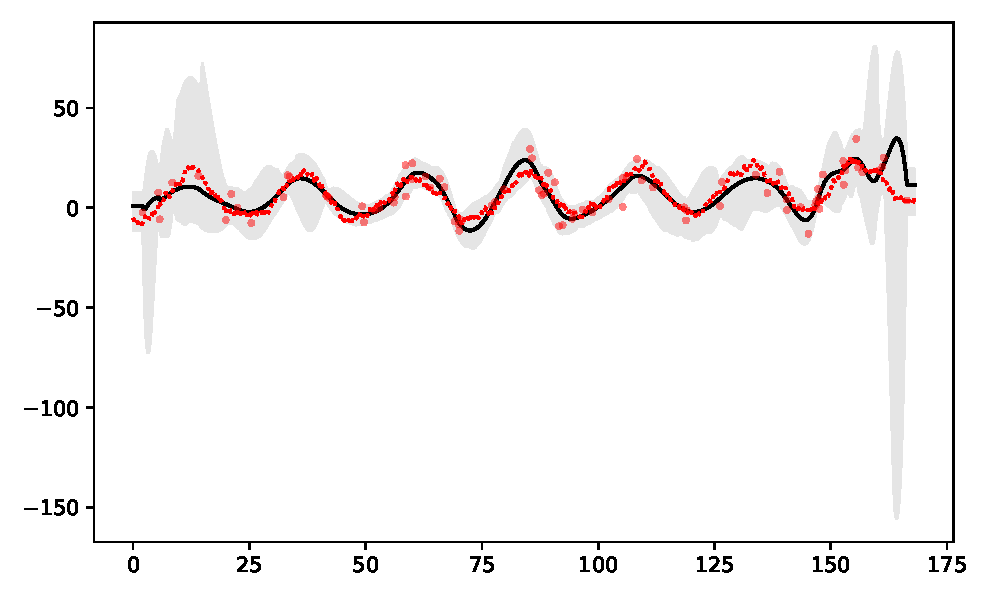
\includegraphics[width=\linewidth]{
        Pictures/plots_final4/sin_rbf_default_0.2/09_12_13_05_43/plot_posterior_confint_spline}
    \caption{Smoothing Spline}
    \label{fig:post-spline}
\end{subfigure}
\caption{Linear Regression and Smoothing spline used
to estimate some example of true BP values $F_X$. The estimated BP values $\hat{F}_X$ (black line), the
        true BP values (red dashed line) and the training data (red dots). The gray area shows
the bootstrap CI.}
\label{fig:regression-example}
\end{figure}


\subsection{Overall Mean}
This method sets $\hat{F}_X$ to the mean of all measurements
$Y_{X_{train}}$ everywhere.


\subsection{Naive TTR}
This method directly estimates the target measures
from the noisy measurements $Y_{X_{train}}$, without estimating $F_X$
first.
The one-hour, one-day, and one-week means were calculated by
taking the mean of the available measurements within the time period.
If no measurements are available within that period, the mean
overall measurements were used.

For calculating TTR, the number of measurements within the range over
the total number of available data points.


\section{Adversarial Analysis}\label{sec:adversarial-analysis}

This section explores the influence of the sampling pattern on the accuracy of
target measure estimates.
As discussed in Section \ref{sec:characteristics-of-the-blood-pressure-time-series},
data density was expected to vary within the Aktiia population,
and measurements were not uniformly sampled.
Instead, data density followed a circadian cycle, referred to as "seasonal sampling."

To create varying levels of data density, downsampling was applied to the dataset
$X$ to obtain $X_{train}$.
Different downsampling factors were investigated, including 20, 10, 5, and 2.5.
A downsampling factor of 20 indicated that $X_{train}$ contained only
5\% of the original data in $X$, which initially had 10 time points per hour.
Consequently, a downsampling factor of 20 or a data fraction of 0.05 implied
that measurements were, on average, taken every other hour.

Seasonal sampling was implemented by extracting the true seasonal component
from the original BP samples. The values of these seasonal components
shifted to contain only positive values and scale to sum up to one,
served as probability weights when selecting data for $X_{train}$ from $X$.
A more extreme seasonal sampling pattern has been produced by
using the squared values of the seasonal component as probability weights.
The decomposed seasonal component and the resulting seasonal sampling are
illustrated in Figure \ref{fig:seasonal-sampling}.




%Finally, we want to study the impact of the sampling pattern on the
%target measure estimates.
%As described in section \ref{sec:characteristics-of-the-blood-pressure-time-series},
%the data density is expected to vary within the Aktiia population, and
%measurements might
%also not be sampled uniformly, but data density might follow the circadian cycle.
%We will refer to the latter phenomenon as seasonal sampling.
%
%Different degree of data density was produced by downsampling
%$X$ to obtain $X_{train}$. The different downsampling factors studied
%are: 20, 10, 5 and 2.5.
%A downsampling factor of 20 implies that $X_{train}$
%contains a fraction of 0.05 of the original data $X$, which contains
%10 time points per hour. A downsampling factor of 20 and a data fraction of
%0.05 therefore implies that measurements have on average been
%taken every other hour.
%
%Seasonal sampling was achieved by extracting the true seasonal component from
%the true BP sample. The values of the seasonal components were used
%as probability weights when choosing $X_{train}$ from $X$. The decomposed
%seasonal component and the resulting seasonal sampling are illustrated
%in figure \ref{fig:seasonal-sampling}.
%

\begin{figure}[!htb]
\centering
\begin{subfigure}{.3\textwidth}
    \centering
    \includegraphics[width=\linewidth]{
        Pictures/plots_final4/sin_rbf_seasonal_default_0.2/09_12_13_15_56/plot_true_mean_decomposed}
    \caption{Decomposed $f(x)$}
%    \label{fig:post-linear}
\end{subfigure}\hfill
\begin{subfigure}{.3\textwidth}
    \centering
    \includegraphics[width=\linewidth]{
        Pictures/plots_final4/sin_rbf_seasonal_default_0.2/09_12_13_15_56/plot_true_with_samples}
    \caption{$f(x)$ and measurments from seasonal sampling.}
%    \label{fig:post-spline}
\end{subfigure}\hfill
\begin{subfigure}{.3\textwidth}
    \centering
    \includegraphics[width=\linewidth]{
        Pictures/plots_final4/sin_rbf_seasonal_extreme_0.2/09_13_07_48_30/plot_true_with_samples}
    \caption{$f(x)$ and measurments from extreme seasonal sampling.}
%    \label{fig:post-linear}
\end{subfigure}
\caption{Panel (b) and (c) show the sample $f(x)$ (red dashed line) drawn from the true GP with measurments generated
by seasonal and extreme sampling (red dots). Panel (a) shows $f(x)$ decomposed into its components.
The probability weights used for downsamplin $X$ are calculated
from the values of the periodic component (orange)}
\label{fig:seasonal-sampling}
\end{figure}



\section{Computational Frameworks}

All code has been written in Python.
For Gaussian process simulation and regression, for fitting the Smoothing Spline
and Linear Regression, the Pyton package scikit-learn
has been used.

%Unless otherwise stated the Pyton package scikit-learn has been used.













